\documentclass[11pt]{article} %This sets the font size and the document class of your report. In this case we use 'article' as that is ideal for shorter reports.
\usepackage{amssymb}
\usepackage{amsmath}

% LaTeX can be enhanced by the use of packages. These packages can do many things, a few of the most common and useful are used here. They are declared before the document proper, in what is known as the 'preamble'. Packages need to be installed when a .tex file compiles into a .pdf, but should do so automatically.

\usepackage[top=2.54cm, bottom=2.54cm, left=2.75cm, right=2.75cm]{geometry} %This sets the margins of the report.

\usepackage{graphicx} % A package allowing insertion of images into the text.

% Choose your citations style by commenting out one of the following groups. If you decide to change style, you should also delete the .bbl file that you will find in the same folder as your .tex and .pdf files.

% IEEE style citation:
\usepackage[style=ieee]{biblatex}
\addbibresource{sem_2_report.bib}

%% Author-date style citation:
%\usepackage[round]{natbib} % A package that creates references in the author-date style, with round brackets
%\renewcommand{\cite}{\citep} % For use with natbib only: comment out for the cite package.
%\bibliographystyle{plainnat} % Author-date referencing (use in conjunction with the natbib package)
\usepackage{color} % Allows the colour of the font to be changed by using the '\color' command: This is just to support the blue comments in this template...use standard (black) text in your report.
\usepackage{float}
\linespread{1} % Sets the spacing between lines of text.
\setlength{\parindent}{0cm}  % Suppresses indentation of text at the start of a paragraph
\pagenumbering{arabic} % sets the style of page numbering for the report


\begin{document} % This begins the document proper and ends the pre-amble

% The last } finishes the chunk of text opening with {\color{blue}..., so all of the above appears as blue text. A common LaTeX error is to forget to close such a chunk of text, so if the formatting goes wrong look for a missing }.

% To get rid of the blue text, select and delete everything from '{\color' to '}', inclusive, leaving \ begin{titlepage} as the first command  after \begin{document}

\begin{center} % Starts the beginning of an environment where all text is centered.

{\Huge Simulating light detection in liquid argon time projection chambers for neutrino and dark matter experiments with deep learning techniques}\\[0.5cm] % [0.5cm] sets the distance between this line and the next.
\vspace{5mm}
\textit{Enrico Zammit Lonardelli}
\\
\vspace{5mm}
\text{9910821}
\\
\vspace{5mm}
\text{School of Physics and Astronomy}
\\
\vspace{5mm}
\text{The University of Manchester}
\\
\vspace{5mm}
\text{Masters Project}
\\
\vspace{5mm}
\text{May 2020}
\\
\vspace{5mm}
This experiment was performed in collaboration with \textit{Krishan Jethwa}\\[0.3cm] % The '\\' starts a new paragraph, and will only work after a paragraph has started, unless we use '~'.

\end{center}
\vspace{60mm}
{\Large \textbf{Abstract}}
\vspace{2mm}
\\
This report details the work done as part of our Masters project, as a continuiation of work done in the first semester.
We discuss quantitative comparisons between the prestablished Montecarlo and novel deep learning methods.
Furthermore, we present the results of our GAN architecture to learn variables of light intensity $S_1$, $S_2$ and $f_{200}$ by implicit learning of their mutual underlying conditional probabilities.
We conclude that the results are INSERT HERE QUANTITATIVE MEASURE OF CONCLUSION.

\pagebreak
\section{Introduction}
\subsection{Problem definition and physics motivation}

\par Cosmological findings have been the driving force for dark matter search for the past X years.
The leap to a Weakly Interacting Massive Particle (WIMP) is not a trivial one and must take great care in assumptions 
it makes and why it makes them, especially in light of increasing ranges of masses excluded by experiments running today.
The first feature of importance is thus mass. 
This is currently under heavy debate in the scientific community as there are supporters of a MILLI mass while on the other spectrum most standard direct
detection experiments today are for ranges running from MASSIVE.
Evidence from phenomena such as gravitational lensing and the constant rotational velocities of stars in galaxies with increasing
distance to their galactic centres suggest a candidate of dark matter halos around these celestial objects.
\\ 
\par From supersymmetrical neutralinos to superheavy dark matter candidates we are looking at a range from GeV/$c^2$ to several TeV/$c^2$ and even higher in certain theories.
What many of these theories have in common however is that they all produced these WIMP candidates as a bi-product or as required assumptions
to allow their theories to work.
This then strengthens the theory that such a particle should exist and also what regions of mass, energy and interaction type to look for.
These WIMPs are hypothesised to have been in thermal equilibrium with thermal plasma in the early universe. 
As the universe expanded and WIMP annihilation rate was less than the Hubble expansion rate, relic density for dark matter was reached.
This brings us to the cross-sections expected for such WIMPs.
Although this varies from theory to theory, we are expecting orders of the weak interaction scale. 
\\
\par This incredibly low interaction rate with regular matter makes it a challenge to detect such WIMPs.
There have been efforts at the Large Hadron Collider to detect missing energies and transverse momenta which could be
explained only through a missing new particle in the mass range of a dark matter candidate.
Although, to date, these efforts have translated into constraints of cross sections and mass the search is still active.
\\
\par Another method of search is through indirect detection by observing celestial objects which have a high mass to luminosity disparity.
These include but are not limited to galactic centres, dwarf galaxies and close galaxy clusters.
This method relies on closely monitoring the particle flux coming from these places waiting for self-interactions or decays into measurable standard model particles to occur.
Searches via these methods are made even harder by the fact that the only biproducts most experiments can reliably measure after accounting
for interstellar magnetic fields, other celestial objects and low background limists are neutrinos and specifi gamma ray energies.
\\
\begin{figure}[H]
\centering
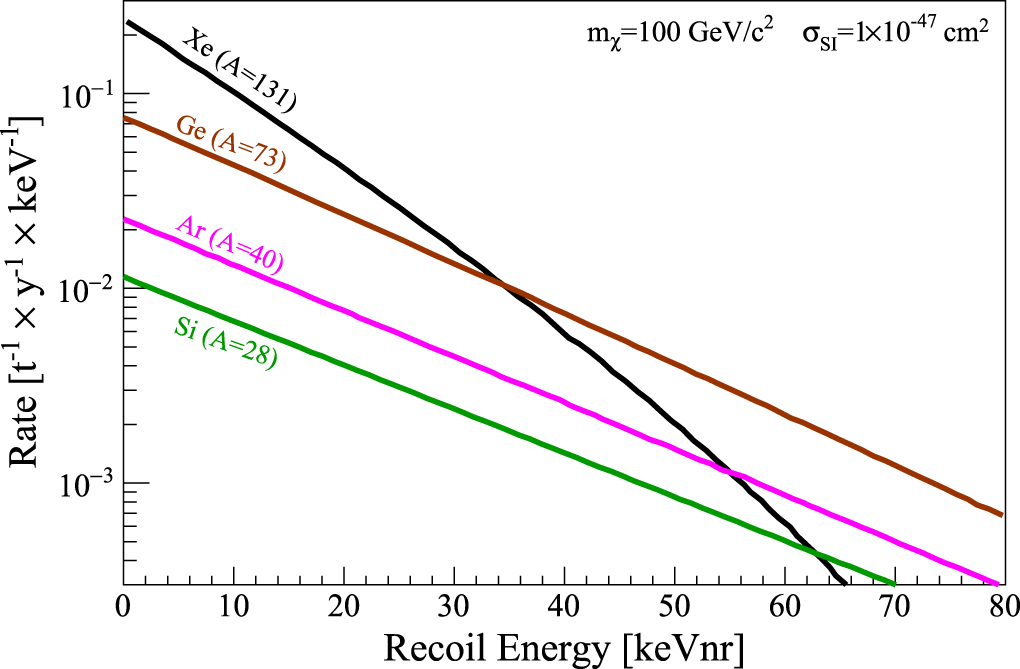
\includegraphics[scale=1]{images/recoil_spectra.jpg}
\caption{\cite{Schumann_2019} Nuclear recoil spctra for varying noble gas targets highlight the better interaction
rate at lower nuclear recoil energies for heavier targets but a lower rate for higher recoil energies.}
\label{fig:recoil_spectra}
\end{figure}
\par Finally, the last method of detection is direct detection.
Large detector chambers are set up, often many kilometers under the earth, essentially waiting for a WIMP
candidate to produce an elastic nuclear recoil with a noble element atom and produce measurable scintillation.
For a WIMP mass ranging between 1 GeV/$c^2$ and 1000 GeV/$c^2$ the recoil energies are in the range 1-100 keV
after which the crossections become way too small for modern detectors.
The choice of noble gas element to use is also non trivial since the rate for spin-indipendent interactions increases with
nucleon number however decreases at high energies due to form factor suppression, as expressed by \cite{lewin1996review} 
\begin{equation}
\frac{{\rm{d}}{R}}{{{\rm{d}}{E}}_{\mathrm{nr}}}\propto \exp (- \frac{{E}_{\mathrm{nr}}}{{E}_{0}} \frac{4{m}_{\chi }{m}_{N}}{{({m}_{\chi }+{m}_{N})}^{2}})
\end{equation}
and shown in Figure \ref{fig:recoil_spectra} for increasing mass of the target nucleus.
\\
\par The higher interaction rate for lower recoil energies makes it more probable to detect a WIMP candidate interaction
however these energies produce a lower intensity of scintillation which results in larger errors
 (from sources such as photomultiplier calibration, photon efficiency, dark currents) so there is a compromise to be made.
These interaction rates are directly relatable to our study in teaching an algorithm the photon efficiency maps of the detector
with varying recoil energies.
With the use of Montecarlo simulators such as G4DS one has to incorporate the nuclear recoil spectrum in the simulation setup
and the program will sample from this the Ar40 recoils accordingly.
This process is a long one since this program simulates everything from the interaction to detection.
This process can take several days if running over many energies with all the scintillation being captured.
\\
\par Similarly, our machine learning algorithm is trained uniformally across the different energies but the choice of 
dark matter regime to be studied can be changed after training directly through the interaction rate distribution by choosing a suitable nuclear recoil spectrum.
This is where the real advantage presented by this deep learning approach comes into play since the training is done once and changing 
sampling distribution can be done virtually instantly and does not require retraining.
\\
\par Finally, to understand the variables of interest in this study consider Figure \ref{fig:detector}.
\begin{figure}[H]
\centering
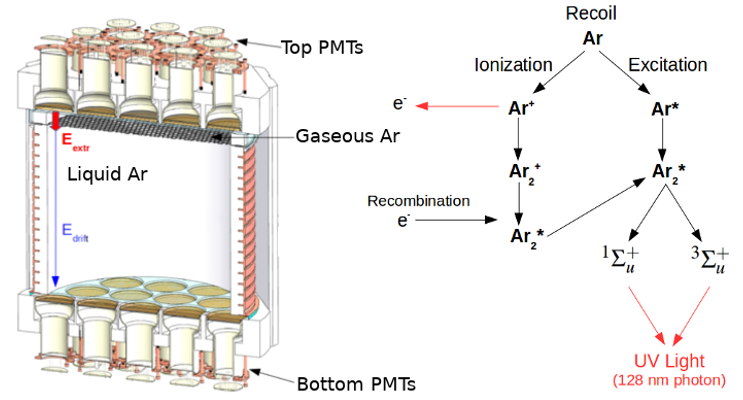
\includegraphics[scale=0.5]{images/detector.png}
\caption{\cite{edkins2017detailed} Schematic of a LAr-TPC and processes of VUV photon emmission.}
\label{fig:detector}
\end{figure}
\subsection{G4DS Results}

\subsection{Deep learning as an alternative}

\section{Methods and Results}
\subsection{Problems in previous work}

\subsection{Novel techniques}

\subsection{Results}
\subsubsection{Variable Learning}

\subsubsection{Analysis and Final Product}


\section{Final Remarks}

\newpage
\printbibliography

\end{document}
